\chapter*{Analysis and Application}
\markboth{Analysis and Application}{Analysis and Application}
\addcontentsline{toc}{chapter}{Analysis and Application}
\thispagestyle{empty}
% <!-- Needs two or three opening sentences -->



This chapter outlines the heuristic for building a predictive maintenance process. It begins by restating the goal of predictive maintenance in precise terms. It then explores data management and feature engineering. The quality of a predictive maintenance process in the photovoltaic domain largely depends on the ability to extract meaningful covariates from the small amount of relevant information. How data should be combined and what methods can be used to improve the quality of covariates is discussed. Then, the data simulation process is returned to, this time with its mathematical underpinnings fully exposed. A comprehensive structure of the simulated data set is provided. Then, a brief introduction to Stan, the probabilistic programming language, is given. This includes a detailed set up of the time-to-event models described in the previous chapter. Finally, the model fit, evaluation and performance are presented.

\section*{The Goal}
\addcontentsline{toc}{section}{The Goal}


The goal of a predictive maintenance process in the photovoltaic domain is to create a system that allows for the correct allocation of maintenance resources regarding inverters with the greatest potential for failure. Formally, this can be seen as creating an sequence of inverters ranked by a score function, $V$, at a given time. Such that:

$$ V_{(1)}(t) > V_{(2)}(t) > \dots V_{(n)}(t) $$

Where the time point, $t$, is fixed at the current moment for prediction. It should be noted, the absolute value of the score is of secondary importance in this process. If maintenance resources are allocated as part of a continuous service it does not matter if the inverter with the highest score is likely to fail within the next day, week or month. It is still the most likely to fail and should still be the inverter to which the maintenance process is applied to first. Therefore, an exact determination of risk is secondary to the action it prompts. This equates time-to-event analysis with rank-order prediction, where the order of failures, and thus the order of maintenance activities are the central goal. 

\newpage
\section*{Feature Engineering}
\addcontentsline{toc}{section}{Feature Engineering}


Feature engineering is sometimes considered the dark art of the statistical modeling process. Its informal nature makes it difficult to find a general consensus as to what the concept actually means within academic literature\cite{Zabokrtsky2015}. Loosely speaking, feature engineering is the art of creating covariates that conceptually embody aspects of a phenomena or object of observation. In this case, it refers to the task of finding and encoding historical information that can describe a photovoltaic inverter's health at any given moment. 

While a multitude of effort is expended generating novel  models which explain and predict better, considerably less attention is focused on what inputs are useful in these models. No domain ever comes with all the ideal features built into existing data sets. Thus, a degree of skill is required to extract and encode what is important. In a practical setting, like the development of a predictive maintenance process, the proper application of feature engineering is the difference between an effective or ineffective method\cite{Yu2010a}. Part of this limited attention stems from the fact that feature engineering is often domain-specific and cannot be adequately generalized. That said, there are themes that can be used to guide the process. The two primary sources of features are subject matter expertise and experimentation. Subject matter expertise can be further subdivided into model-specific and domain-specific insights.

An understanding and awareness of the details and limitations of the model is paramount to being able to create covariates that act as effective inputs. This requires subject matter expertise, which arises from knowledge of the functional attributes of the applied model, such as that presented in the previous chapter. Such knowledge can avoid the negative consequences of using data that may be suboptimal in combination with certain models. For example, when introducing maintenance logs as a time-dependent covariate, it is not sufficient to simply provide a binary variable that records whether an inspection occurred on a specific date. The functional form of the model implies such a formulation is unlikely to serve as a sufficiently strong signal for the effect of regular inspection on lifetimes, as it lacks variability. However, the number of days since the last inspection is more likely to have a substantive effect. The functional structure of the model reveals these conditions and should be kept in mind when constructing covariates.

Domain-specific subject matter expertise is an inescapable necessity for effective feature engineering. While there continues to be a drive toward greater automation in determining the relevance of covariates, human decision continues to remain paramount. In this area, domain-specific subject matter refers to an understanding of the contributing events that lead to failure in photovoltaic inverters. This includes knowledge about the various failure modes of an inverter and their origins. This includes such sources as high voltage, extreme temperatures, water condensation, the lack of robust software by certain manufacturers and others factors. It also includes knowledge about the hardware itself and which components are under stress and contribute to failure, such as capacitors, semiconductor switches and housing materials\cite{Flicker2014}. Domain-specific knowledge provides the necessary scope with which to limit the search for features. It is often best generated from continuous interactions with front-line workers on the system in question.

Experimentation is the last source of feature engineering and is meant to complement rather than substitute subject matter expertise. As its name suggests, this is where features are created and then tested to see whether or not they improve model performance. This includes experimenting with feature encodings, such as making use of power transformations as well as variable discretization, standardization and normalization. All of these changes can potentially improve model performance. It may also include generating new features based on an assumption of effect. For example, it may be wise to include a feature that encodes days with both low temperature and low humidity which can cause printed circuit boards to crack. Then this covariate should be tested to see if it improves predictive performance. 

As feature engineering is more an art-form than a science, there is no single correct method for performing the task. Despite the lack of a clear heuristic, there are some guidelines for introducing features in time-to-event models. An important condition to keep in mind is that time-to-event models have difficulty in dealing with noisy variables across small intervals. The purpose of these models is to determine the contribution of covariates to the rate of failure. However, the introduction of stochastic variables, such as daily temperature, may not have that desired effect. This is because the effect of temperature on an inverter is only relevant in certain extreme cases over time and not in any one case. The effect of a single day of extreme temperature is unlikely to result in a failure on that day. In effect, this violates the association that the model demands between covariate value and inverter status. This can be partially offset by the use of rolling aggregates, that provide an average temperature over a specific intervals. However, by definition, these extreme events are rare, and will likely be smoothed out in these rolling aggregates. Furthermore, this does not account for compounding effects. A better solution is the use of monotonically increasing variables like a count of extreme temperatures across a specific interval. Of course, such a feature requires a definition for 'extreme', one which should be subject to experimentation on a validation set. Yet, it is important to realize that time-dependent variables require trajectories to be utilized effectively for predictive purposes. 






\section*{Data Management and Simulation}
\addcontentsline{toc}{section}{Data Management and Simulation}


Raw data can rarely be input into a model as-is. The first chapter broadly examined the standard data sources for a predictive maintenance process as well as provided a general outline of the simulated data. This section returns to these topics and examines the structure of the input data. It then turns its attention to the process of data simulation, introducing the quantile function and the inverse cumulative hazard. Finally, it presents the data used in the subsequent analysis.


Data required for a predictive maintenance process often comes from several different database tables meant to record different aspects of a collection of systems. This includes databases that document system attributes, maintenance and failure history and condition monitoring and usage patterns. Conversely, time-to-event models, require a form of attribute-value data. This data format can be roughly thought of as tabular data. Each row is a system, and each column encodes a covariate, with one column containing the failure status of the system. The input data then provides a table of the last observed value of each system and their respective covariates. These values can then be transformed into a table which can be fed into Stan. 



\begin{figure}[htbp]
  \centering
    \begin{tabular}{l|l}
    \textbf{Covariate/Feature} & \textbf{Description} \\
    \hline
    time  & observed time \\
    censor & censoring indicator  \\
    id    & unique identifier for inverter \\
    park  & unique identifier for park \\
    type  & inverter type: central string or micro \\
    kWh\_l30d & average kwh in last 30 days standardized \\
    weather\_l6m & count of extreme weather events in last 6 months \\
    err\_code01\_l30d & count of minor errors in last 30 days \\
    err\_code02\_l30d & count of major errors in last 30 days \\
    repair\_days & days since last repair \\
    \end{tabular}%
  \caption{Covariates/Features of Simulated Data}
  \label{dat_vars}%
\end{figure}%



Figure~\ref{dat_vars} gives an illustration of how data should be structured on input. The suffix, 'l30d' takes the count in the last thirty days of operation of a particular value, such as 'kWh' which encodes outlying energy output or 'weather' which encodes extreme weather events. The suffix, 'days', counts the number of days since an event, in this case the number of days since any repair was performed on the inverter. 

Recall that the input for the models was structured as follows:

$$ (Y_ij, d_{ij}, Z_i,  \textbf{x}_{ij}) $$

In this case, the observation time is $Y$, the censor indicator is $d$, the park is the Frailty, $Z$, and the remaining variables make up, $\textbf{x}$. It should be noted that this data is an example of what should arise after the feature engineering process is complete. That said, this is far simpler data than what would result from a real-world setting and is meant for illustration purposes. The goal is to produce a set of covariates that can adequately represent the failure mode of a device in order to enhance the understanding of the model not to necessarily replicate all the nuance of the real-world.

Data is simulated using inverse transform sampling. This method generates random values from any distribution using only standard uniform random values as inputs. Generally speaking, this enables the generation of values from any continuous distribution. 

Briefly, let $F$ be a continuous cdf. This guarantees that $F^{-1}$ exists as a function from $(0,1]$ to $\mathbb{R}$. If $U$ is defined as a uniform random variable on the unit interval, $(0,1]$ and $T = F^{-1}(U)$, then $T$ is a random variable with the cdf, $F(\cdot)$. As the function of a random variable is also a random variable itself, the inverse of the cdf, $F^{-1}(U)$, known as the quantile function, is also a random variable\cite{Blitzstein2014}. This implies that, $F^{-1}(U) = T$ if and only if $U = F(T)$. Thus, all that is required to generate random values from any given distribution is the quantile function and uniform random variables. 

In this case, there is a desire to generate survival lifetimes. In the previous chapter, the cdf of a general lifetime distribution was given as follows:

$$ F(t) = 1 - S(t) = 1 - \exp(-H(t)) $$

Due to symmetry, a uniform random variable is defined on the unit interval for the survival function as well as the cdf. If $U \sim \text{Unif}[0,1]$ then $(U-1) \sim \text{Unif}[0,1]$ as well. Thus:

$$ U = \exp(-H(T)) \sim \text{Unif}[0,1] $$

As long as all hazards are defined to be strictly positive, $h(t) > 0$, the cumulative hazard, $H(t)$ is invertible and the survival time can be expressed as:

$$ T = H^{-1}(-\ln(U)) $$

Fortunately, for all of the models presented thus far an inverse of the cumulative hazard exists. From this starting point it is possible to generate models with considerably more complex features.

For the Multiplicative Hazards Model with covariates, survival times are generated the following manner\cite{Bender2005}:

$$ T = H_0^{-1}(-\ln(U) \exp(-\boldsymbol\beta^T \textbf{x})) $$

Where $H_0^{-1}$ is the inverse of the baseline cumulative hazard function which is multiplied by the exponentiated effect of the covariates. 

This simulation can be extended further to include the a Frailty term, $Z_i$, it then becomes\cite{Romdhane2015}:

$$ T = H_0^{-1}\left [\frac{-\ln(U)}{Z_{i} \exp(\boldsymbol\beta^T \textbf{x}_{ij})}  \right ] $$



Of course, the precise model depends on the parameterization of the baseline cumulative hazard. As stated in the previous chapter, numerous different distributions can be used for modeling lifetimes and any of them can be used for this baseline cumulative hazard. In this case, a Weibull baseline hazard is employed. The resulting model with shared Frailties can therefore be simulated as follows:

$$T = \left [\frac{- \ln(U) }{Z_{i} \gamma^{-\alpha}  \exp(\boldsymbol\beta^T \textbf{x}_{ij})}  \right ]^{1/\alpha} $$

Where $u$ is the realization of a uniformly distributed random variable, $U \sim \text{Unif}(0,1]$ and $\alpha$ and $\sigma$ are the shape and scale parameters of Weibull distribution, respectively.



\section*{Evaluating Model Performance}
\addcontentsline{toc}{section}{Evaluating Model Performance}


Time-to-event models focusing on predictive outcomes create a unique problem for evaluating performance. On one hand, the output of the model creates hazards, which are continuous and have a support on all positive real numbers $[0, \infty)$. In parametric models, these hazards are monotonically related to expected residual lifetimes. So an estimate of the difference between the hazard and observed remaining lifetime could be used to assess model performance. On the other hand, a determination of the exact failure time provides more information than is required for the task, not to mention censorship makes the real lifetime difficult to observe in many cases. Knowledge of the order in which failure occur is generally sufficient to schedule maintenance activities. This is especially true given the limited amount of information available in photovoltaic systems. 

This section provides the basis for evaluating performance of time-to-event models for predictive outcomes. It begins by discussing the goal of model performance and addresses the difficulties that arise from applying traditional model evaluation techniques in the time-to-event context. It then introduces the Concordance-Index (C-Index) as well as the Widely Applicable Information Criterion (WAIC) which are used for model discrimination and calibration. Finally, a general heuristic is provided for evaluating performance in this class of models.

Ideally, a well-performing time-to-event model should behave in a manner that generalizes the relationship between the covariates and the lifetime. After all, the purpose of any model is to discover the patterns that reveal the phenomena generating a class of data rather than any specific data set. Thus, a well-tuned model of lifetimes should apply to observations of new photovoltaic inverters just as well as it does to those already in operation. To assess this generality, it is important to ensure that the model performs well out-of-sample. Failure to do so can result in underfitting or overfitting, both of which are detrimental aspects of model performance. 

Underfitting refers to when a model is unable to capture the complexity of the underlying phenomena. This is caused by the sin of omission, such as when important structural features or relevant covariates are not included in the model. As a result, the model is inflexible and will systematically bias results both in and out-of-sample. This is because underfitting results in an insensitivity to the structure of any sample. Overfitting refers to when random variation is treated as structure by a model. In an extreme case, overfitting can be thought of as data memorization. Thus the model memorizes the sample used to fit it. This makes it incredibly accurate in-sample. However, since new data is unlikely to have the exact same configuration as any single sample, it would result in poor out-of-sample, or generalized performance. Broadly speaking, the difference between underfitting and overfitting rests in the complexity of the model as well as the sensitivity of that model to the exact composition of the sample used to fit it\cite{McElreath2016}. 



As both underfitting and overfitting affect out-of-sample performance, it is important to utilize a metric that takes into account the generality of the model. One of the most common methods to do so in a predictive context is k-fold cross-validation. In the simplest version of the technique, the data is randomly split into $k$ equal sized samples. Then, the model is fit on $k-1$ samples, with the remaining one being used to evaluate out-of-sample performance. This evaluation usually takes the form of mean-squared error (MSE) or mean-absolute error (MAE), both of which measure the distance of predicted values to the observed values in the $k^{th}$ sample. This last sample is not used to fit the model thus acts as a replacement for out-of-sample data. An average of the MSE or MAE can then be taken to provide the general performance of any model. 

Unfortunately, with time-to-event data, k-fold cross-validation becomes difficult to apply. The process has an implicit assumption that each observation is independent and therefore can be randomly split into $k$ samples. In a time-to-event context, the sequence of lifetimes is of importance. As such, this method would result in historical information about a lifetime being randomly excluded from model fitting. The result would be a systematically underfitting of the baseline hazard. It would also increase deviations from the real hazard over time, as changes in initial conditions would result in greater deviations from the true hazard as time progresses.


Censoring also creates problems for this technique. It results in data that is severely unbalanced. Very few industrial settings feature an abundance of failures. Decades of reliability engineering has ensured that most industrial systems are not prone to widespread failure. Photovoltaic inverters are not excluded from this generalization\cite{Petrone2008}. As a result, the majority of observations will be non-events. While all observations may eventually become events, as all systems eventually break down, it is highly unlikely in a production setting that the data will be balanced. Datasets where the majority of observations are non-events are the rule in time-to-event contexts, not the exception. As a result, the balanced comparison of predicted to observed lifetimes is difficult as that data makes up such a minor proportion. 

In the time-to-event context, the Concordance Index (C-Index) can serve as a reasonable measure of the predictive performance of a model. It is commonly used in prognostic studies in the medical domain\cite{Tripepi2010}. The C-Index is the conditional concordance probability measure of a lifetime and a predictive score variable\cite{Kang2015}. In this case, the predictive score is the hazard, as it estimates the risk a system is in at a given time. The C-Index compares the relationship between the actual lifetime and the hazard of a particular model. Its computation is also relatively straight forward and is capable of being extended to include censorship.

In the case for non-censored observations, the following applies: Let $(t_i, h_i)$ be the observed time and hazard of an individual system, $i$, in a collection of $n$ systems.

Probability of concordance is defined as:

$$\mathbb{P}_c  = \Pr(t_i  < t_j \text{ AND } h_i < h_j \text{ OR } t_i  > t_j \text{ AND } h_i > h_j)  $$

Probability of discordance is defined as:

$$\mathbb{P}_d  = \Pr(t_i  < t_j \text{ AND } h_i > h_j \text{ OR } t_i  > t_j \text{ AND } h_i < h_j)  $$

Then, generally the C-Index is:

$$ C_{t, h} = \frac{\mathbb{P}_c}{\mathbb{P}_c + \mathbb{P}_d} $$

As can be seen from the above, the C-Index is simply the fraction of concordant pairs to all pairs. Put another way, it is the proportion of times the hazard correctly orders the lifetime of a system. Of course, the above is only applicable if all lifetimes are observed and, as noted earlier, this is rarely the case. However, to extend the C-Index to censored observations a more imperative version of the above is required. 

\begin{figure}[ht!]
    \centering
    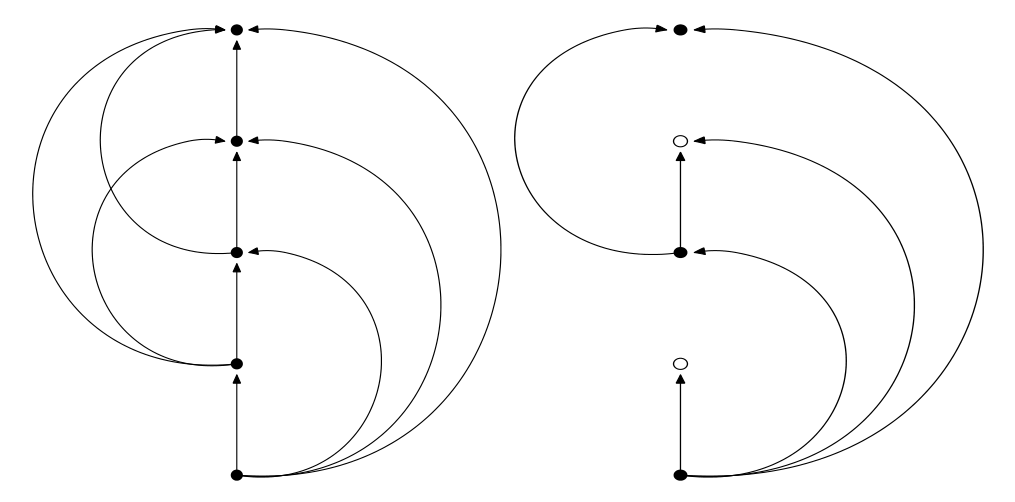
\includegraphics[width=350pt]{img/c_index_graph}
    \caption{Order Graph of C-Index Without and With Censoring}
    \label{ci_graph}
\end{figure}


To introduce the effect of censored observations, it is easier to think of time-to-event data as an ordered graph, $\mathcal{G} = (\mathcal{V}, \mathcal{E})$, and as displayed in Figure~\ref{ci_graph}\cite{Steck2008}. Each observation is a triple, $(t_i, h_i, d_i)$, with the observed time, hazard and censoring indicator for any individual system. The set of vertices $\mathcal{V}$ represent all individual triples in the data set. Each vertex, $\mathcal{V_i}$, is indicated to be either an event or censored using the censoring indicator, $d_i$. Edges, $\mathcal{E}_{ij}$ between the vertices of the graph are only drawn such that $t_i < t_j$ and no edges can come from a censored observation.

In such a context, the C-Index is:

$$ C(t, h, d, \mathcal{G}) = \frac{1}{\mathcal{|E|}} \sum_{\mathcal{E}_{ij}} I(h_i < h_j) $$

With $I(\cdot)$ being the indicator function, which is one if $h_i < h_j$, and zero otherwise. The $\mathcal{|E|}$ is the number of edges in the graph.

It is important to take a moment and understand what this construction implies. Censored observations contribute to the C-Index only in one direction. Specifically, if and only if, an uncensored failure time is smaller than a censored survival time. This makes intuitive sense. If a pair of observations are given, $i,j$, where $t_i < t_j$, then if the first observation, $i$, is an event it can still be compared to the censored observation later in time. If the score of the first observation is larger, then a concordant pair results, if not, the result is a discordant pair. However, if the first observation is censored, nothing can be said about the pair. This is because, by definition, a censored observation will have a lifetime greater than that of an event. So there is nothing to determine whether that censored observation will continue to survive until it has a lifetime less than or greater than the event observation. 

The C-Index can have this one-directionality made more explicit in the following way\cite{Steck2008}:

$$ C(t, h, d, \mathcal{G}) = \frac{1}{\mathcal{|E|}} \sum_{t_{i}|d_i = 1} \sum_{t_i < t_j} I(h_i < h_j) $$

The C-Index is a generalization of the Area Under Curve (AUC) or the Receiver Operating Conditions (ROC) plot, both of which assess the predictive performance of a binary classifiers\cite{Cook2007}\cite{Tripepi2010}. Clearly in this context, the goal is not binary classification, rather the correct ordering of events. However, a similar interpretation result occurs as in other contexts. The C-Index has a range of $[0.5,1]$. At one extreme a C-Index is one, which implies the model produces a perfect prediction, such that the rankings of each hazards are concordant with each lifetime across all observations. At the other extreme, $0.5$, the model has a probability equivalent to flipping a coin. 


The C-Index does have its drawbacks. While the C-Index has objective value as a metric for establishing the predictive accuracy of a model, it is less suitable for selecting which set of covariates produce the best model. This is because it is relatively insensitive to the inclusion of covariates\cite{Cook2007}. Different sets of covariates are unlikely to result in substantial changes in the C-Index's numerical value. The lack of substantial variation can make the task of model selection somewhat more difficult. Thus, it is important to complement the C-Index with more traditional methods of assessing the goodness-of-fit of a model. Highly recommended are the use of methods that derive out-of-sample deviance based on Information Criteria. 

In the Bayesian context, the Widely Applicable Information Criterion (WAIC) is a novel metric that provides point-wise average out-of-sample deviance\cite{Watanabe2010}. The WAIC is an improvement over the Deviance Information Criterion (DIC) which is commonly used in Bayesian analysis. It addresses several of the shortcomings that are associated with this metric, mainly stemming from the DIC being computed around a point estimate. 

Briefly, the WAIC approximates the expected log posterior predictive density for a new dataset\cite{Vehtari2015}. 

$$ \text{elpd} = \sum_{i=1}^n \int p_t(\tilde{y_i})\ln p(\tilde{y}|y) d\tilde{y}_i $$

Where $p(\tilde{y}|y) = \int p(\tilde{y}|\theta)p(\theta|y) d\theta$ is the posterior predictive distribution and $p_t(\tilde{y_i})$ is the distribution of the true data generating process. Clearly, the true data generating process is not observed. However, it can be approximated the following way:

$$\hat{\text{elpd}} = \hat{\text{lpd}} - \hat{p}$$

Where $\hat{\text{lpd}}$ is the log pointwise predictive density and the $\hat{p}$ is the number of effective parameters in the model. The log pointwise predictive density is simply the probability of observing each one of the data values given the set of parameter values used in the model.

$$ \text{lpd} = \sum_{i=1}^n \ln \int p(y_i|\theta)p(\theta|y) d\theta \qquad \hat{\text{lpd}} = \sum_{i=1}^n \ln\left ( \frac{1}{S} \sum_{i = 1}^S p(y_i|\theta^s)  \right ) $$

Where $\theta^s$ is the vector of completed posterior simulations. 

The effective number of parameters is approximated using the sample variance of the log likelihood of posterior distribution.

$$ \hat{p} = \sum^n_{i=1} \text{VAR}[\ln p(y_i|\theta^s)] $$

Where $Var[\cdot]$ is the sample variance.

This entire process is easily implemented in Stan as it can be directly computed in the \lstinline{generated quantities} block\cite{Vehtari2014}. As with all information criterion metrics, the lower the value the less deviation there is from the true data generating distribution. 

The C-Index and WAIC evaluate performance but through different means. Both assess the generalization of the model to new data. But both have substantially different practical interpretations. Yet, if the model is stable, both should result in the same conclusion being reached about accuracy and discrimination. Yet, if an error in model design or fit has occurred, their lack of harmony should be a signal to reevaluate the current model. 



\newpage
\section*{Stan}
\addcontentsline{toc}{section}{Stan}


Stan is the most recent addition to the toolkit for fitting Bayesian models. Like its predecessors, BUGS and JAGS, Stan seeks to abstract the task of fitting complex models with a general programmatic process. Stan makes use of Hamiltonian Monte Carlo (HMC) for the sampling of continuous parameters from a model. The existence of Stan stems from the operational difficulties of its predecessors in dealing with multilevel generalized linear modeling contexts. These software packages have requirements, such as conjugate priors or log-concave posterior densities, for models. This made anything outside of those rigid constraints incredibly inefficient when sampling was performed. In the current context, the introduction of complex shared Frailties can create similar problems with these existing modeling tools. 

A Stan program defines a statistical model through a conditional probability function, $\Pr(\theta|y,x)$, where $\theta$ is a sequence of unknown modeled values while $y$ is composed of modeled known values, and $x$ of unmodeled covariates and constants\cite{StanDevelopmentTeam2016}. Stan is an imperative probabilistic programming language. This implies that the language requires the user to tell it how to do something more than just declare that it should be done. Precise instructions have to be written verbatim to achieve the desired modeling outcome. Yet, as the previous chapter demonstrated, models are constructed by combining relatively simple building blocks. This permits models of any complexity to be defined and built upon.


\begin{figure}[htbp]
    \centering
    \begin{lstlisting}[belowskip=-2 \baselineskip]
        functions {
        	// ... function declarations and definitions ...
        }
        data {
        	// ... declarations ...
        }
        transformed data {
        	// ... declarations ... statements ...
        }
        parameters {
        	// ... declarations ...
        }
        transformed parameters {
        	// ... declarations ... statements ...
        }
        model {
        	// ... declarations ... statements ...
        }
        generated quantities {
        	// ... declarations ... statements ...
        }\end{lstlisting}
    \caption{Available Stan Blocks}
    \label{stanblocks}
\end{figure}


A Stan program consists of variable declarations and statements, divided into a series of blocks written in a C-like syntax. This compartmentalizes operations, as variables can be declared in the block within which they are used. Generally, three blocks are used to define a statistical model. These are the data, parameters and model blocks. Figure~\ref{stanblocks} demonstrates all the available blocks and their required order.

The data block declares the data required for the model. The parameter block declares the model parameters, or the unobserved random variables being sampled by the model. The model block defines the log probability function used to fit the model. 

The data and parameter blocks both handle declaration of variables. In Stan, random variables are handled differently depending on whether or not they are observed. Observed random variables are declared as data while unobserved random variables are declared as parameters. Unobserved random variables can be sampled from or inserted in subsequent blocks. This is especially useful in the computation of the log probability function. 

To facilitate processing two transformation blocks and generated quantities block are available. The transformation blocks allow for data and parameters to be altered and saved in the process of executing a Stan program. This provides additional flexibility in model building. The generated quantities block allows for the creation of values of importance, such as summary statistics. The block is run at the end of each sampling step, this permits for the tracking of intermediary values as the model is fit. 

Once a Stan program is defined, it is compiled into \lstinline{C++} code before being executed. The program begins by validating the known values of $y$ and $x$ and checking their types and constraints. It then generates a sequence of non-independent identically distributed parameter values, which have a marginal distribution of $\Pr(\theta|y,x)$. This translation into \lstinline{C++} code greatly improves the speed and portability of Stan-built models. However, it also results in requirements that do not arise in earlier Bayesian samplers. Notably, Stan is statically typed and requires that all variables have their constraints explicitly defined, if they exist. This is partially to enforce explicitness among model designers, but it is also to prevent modeling errors from creating problematic outputs. For example, a Weibull baseline hazard requires that both the shape and scale parameters be strictly positive otherwise the function is not defined. There is no reason for any sampler to make use of negative parameter values when sampling from these distributions. Strict type setting with constraints ensures that these types of errors are caught as soon as they occur rather than potentially disturbing final results. 

Once the sampler runs until convergence, Stan writes the output values of each parameter to disk in a \lstinline{csv} file. This permits sampling to be done multiple times with the values of each iteration updating the output. This is particularly useful for large models that may require a greater amount of computer time for each iteration.

Stan comes with a great many of built-in operations and functions. The basic operations are the same as one expects from any programming language, logical and arithmetic operations, matrix and array manipulation, type conversions as well as built-in functions for handling mathematical operations like solving ordinary differential equations. The language also includes functions that encode most statistical distributions including those that are found in the previous chapter. Furthermore, sampling statements are used that vectorize the sampling from known distributions improving the speed of execution. 

While these built-ins are useful for the vast majority of tasks, time-to-event models pose a problem for 'vanilla' Stan. Much of the difficulty in building time-to-event models in Stan stems from the presence of censoring and truncation in the data. While Stan does have some support for dealing with censoring and truncation, the nature of this support is fairly inflexible, especially when dealing with more complex models, such as those with time-dependent variables or Frailties. The recent introduction a function block in the language has largely enabled the fitting of time-to-event models in Stan. As the name suggests, the function block allows for any arbitrary function to be declared. This includes the ability to explicitly define a likelihood function. This mechanism permits the development of time-to-event models as the effect of censoring can be written explicitly into the models. 


\section*{Building The Model}
\addcontentsline{toc}{section}{Building The Model}


This section brings all the previous insights together and provides a step-by-step process to fitting and evaluating time-to-event models. It begins with the construction and output of a simple Multiplicative Hazard Model, it then extends to this model to accommodate shared Gamma Frailties. The emphasis in this section is on practical exposition, over theory. As a result, some implementation details may be omitted for the sake of brevity. 

It is important to start simple with model construction. A good first step is to fit a basic Multiplicative Hazards Model, in this case with a Weibull baseline hazard. 

\begin{figure}[htbp]
    \centering
    \begin{lstlisting}[belowskip=-2 \baselineskip]
functions {
  real log_h_t(real lifetime, real alp, real gam);
  real H_t(real lifetime, real alp, real gam);
 
  real log_h_t(real lifetime, real alp, real gam){
    return log( (alp/gam) ) + (alp - 1) * log( (lifetime / gam) );
  }
  
  real H_t(real lifetime, real alp, real gam){
    return ( (lifetime / gam) )^alp ;
  }
  
  real surv_dens_log(vector cens_lifetime, real alp, real gam, real lin_pred){
    real lifetime;
    real d_i;
  
    lifetime <- cens_lifetime[1];
    d_i      <- cens_lifetime[2];
  
    return d_i * (log_h_t(lifetime, alp, gam) + lin_pred) - H_t(lifetime, alp, gam) * exp(lin_pred);
  }
}\end{lstlisting}
    \caption{Function Block for Multiplicative Hazard Model}
    \label{mhazm_funs}
\end{figure}


Stan permits the inclusion of arbitrary functions. These functions can be used in any manner, but in this context they are primarily useful for evaluating the likelihood of the model. To be included, they must be placed in a \lstinline{function} block at the beginning of the model code. Figure~\ref{mhazm_funs} contains code block for the functions needed to define a Multiplicative Hazard Model in Stan. The conditional cumulative hazard, $H(t|x)$, and the conditional log hazard, $\ln(h(t|x))$, are defined in the \lstinline{H_t()} and \lstinline{log_h_t()} functions, respectively. The model's log likelihood, $\ell(\theta|Y, d)$ is defined in the \lstinline{surv_dens_log()} function. This last function that will be minimized in sampling steps of the fitting process. 

The process of explicitly writing likelihoods exposes one to the inner operation of a model. This fosters a deeper connection between the mathematics and programming. Furthermore, such a process enables one to extend the model far beyond what is covered in this text.

It should be noted, that this type of functional definitions are not commonly required to use Stan, as it comes with a large library of built in functions\cite{StanDevelopmentTeam2016}. However, Stan's handling of censored data is currently problematic for most time-to-event models making such functions mandatory. To make the effect of censoring explicit, the likelihood function takes a vector as input \lstinline{cens_lifetime} that contains the double, time and censoring indicator, $(Y_i,d_i)$, needed to define an observed lifetime. 

Stan is statically typed and forces precision in definitions. As a result, every function and variable must have its type explicitly stated before hand. These are provided in Figure~\ref{mhaz_data}. Most common data types are available, including ones for dealing with vector and matrix operations. As these functions deal with continuous variables, \lstinline{real} is the common type. Due to the language's imperative nature, order is not arbitrary and all variables and functions must be defined prior to being used. 


\begin{figure}[htbp]
    \centering
    \begin{lstlisting}[belowskip=-2 \baselineskip]
		data {
		  int<lower=0>  N;
		  vector[2]     lifetime[N];
		  real          x_err1[N];
		  real          x_err2[N];
		  real          x_repair[N];
		  real          x_kWh[N];
		  real          park_weather[N];
		}\end{lstlisting}
    \caption{Data Block for Multiplicative Hazard Model}
    \label{mhaz_data}
\end{figure}


To allow for the sampling of the likelihood, input data must be defined. These are the observed values. Data can be input any number of different ways. Stan is self-sufficient and it can be accessed through a variety of programming languages, like R, Python, Julia, etc. Each one of these languages have the ability to feed data into Stan. In the R language, this is done through a named \lstinline{list()} The names within the list should correspond to the variable names found in the \lstinline{data} block in Figure~\ref{mhaz_data}. The number of observations, the values of those observations and the values of any covariates must be defined here. Note, that the type and dimensions of each element of data must be declared here. It is good practice to center and scale data prior to input. Even if a covariate is a count, like the number of days since repairs or a count of error codes, it is advisable to scale and convert it to real values. This greatly improves the performance of Stan, as HMC is optimized to operate on continuous functions. If this is not done a much slower discrete optimization process is used. Of course, caution is advised as it is possible that the data one wishes to import cannot take on real values. 


\begin{figure}[htbp]
    \centering
    \begin{lstlisting}[belowskip=-2 \baselineskip]
parameters {
  real<lower=0> alp;
  real<lower=0> gam;
  real          beta_err1;
  real          beta_err2;
  real          beta_repair;
  real          beta_kWh;
  real          beta_weather;
}\end{lstlisting}
    \caption{Parameters Block for Multiplicative Hazard Model}
    \label{mhaz_params}
\end{figure}


The parameters of the model also must be defined. This is done in Figure~\ref{mhaz_params}. In this case, this includes the parameters for the Weibull distribution, \lstinline{alp} and \lstinline{gam}, as well as the linear coefficients, \lstinline{beta_}, associated with the model covariates. Notice the \lstinline{real<lower=0>} in the parameter definitions. These are constraints which are applied to the \lstinline{alp} and \lstinline{gam} parameters to ensure that their support is only over the positive real numbers. In this model, failure to do so will result in errors produced by negative probabilities, causing proposal moves to be discarded. This may result in poor convergence and biased parameter estimates. Even in situations where where the sampler does not explicitly warn about negative probabilities, it is best practice to apply constraints if one is aware of them.

\begin{figure}[htbp]
    \centering
    \begin{lstlisting}[belowskip=-2 \baselineskip]
model {
  for(i in 1:N){
    lifetime[i] ~ surv_dens(alp, gam, beta_err1 * x_err1[i] + beta_err2 * x_err2[i] + beta_repair * x_repair[i] + beta_kWh * x_kWh[i] + beta_weather * park_weather[i]);
  }

  alp ~ lognormal(0, 1.5);
  gam ~ lognormal(0, 1.5);
  
  beta_err1 ~ normal(0, 1);
  beta_err2 ~ normal(0, 10);
  beta_repair ~ normal(0, 1);
  beta_kWh ~ normal(0,10);
  beta_weather ~ normal(0, 1);
}\end{lstlisting}
    \caption{Model Block for Multiplicative Hazard Model}
    \label{mhaz_model}
\end{figure}


The model block encapsulates the high-level configuration of the model and defines the sampling process. Figure~\ref{mhaz_model}, defines both the priors as well as the method of sampling. The sampling is declared through a sampling statement. The \lstinline{for()} loop iterates over each element in the data and declares that each observation is distributed, $Y \sim \mathcal {L}(\theta)$,  given a likelihood. In this case, as a log-likelihood was already defined in the \lstinline{function} block it is possible to make use of it. Note that the function being called is \lstinline{surv_dens} not \lstinline{surv_dens_log} as was defined in the \lstinline{function} block. This is because each observation is defined according to the likelihood, even if the model is fit using a log-likelihood. Stan understands the \lstinline{_log} suffix and acts accordingly. This is meant to ensure that the focus is retained on the characteristics of the model rather than its fitting process. 

Below the sampling statement are the priors associated with the parameters. Priors do not have to be explicitly defined in Stan. If they are not, Stan will use a continuous uniform prior. However, these are highly inefficient especially if no constraints were declared for a particular parameter. The consequences of this omission can be poor convergence and biased estimates. This is especially true of the scale parameter of the Weibull distribution, \lstinline{gam}, whose true value is often far from zero. Weakly regularizing priors centered near zero are advisable, especially if all the variables were scaled beforehand. If there is some existing knowledge about the expected lifetime of a system, a prior can also be used as a means by which to introduce this expertise into the model. 



\begin{figure}[htbp]
    \centering
    \begin{lstlisting}[belowskip=-2 \baselineskip]
generated quantities {
  vector[N] pred_log_h_t;
  for(i in 1:N){
    pred_log_h_t[i] <- log_h_t(lifetime[i,2], alp, gam, beta_err1 * x_err1[i] + beta_err2 * x_err2[i] + beta_repair * x_repair[i] + beta_kWh * x_kWh[i] + beta_weather * park_weather[i]);
  }
}\end{lstlisting}
    \caption{Generated Quantities Block for Multiplicative Hazard Model}
    \label{mhaz_quants}
\end{figure}

Lastly, it is possible to directly output the posterior predictive distribution for each inverter using the \lstinline{generated quantities} block. This is shown in Figure~\ref{mhaz_quants}. To achieve this, a simple iteration across each observation using the final parameters is done. These values can then be extracted into R and their predictive accuracy assessed. Most importantly, it is possible to extract the variances on each prediction, allowing this to be taken into account when planning maintenance scheduling. Generally, Stan provides an entire class of functions for numerous distributions with the suffix, \lstinline{_rng} that allow for the generation of these quantities. However, as a custom likelihood is used, so too must a custom range function.

\begin{figure}[htbp]
    \centering
    \begin{lstlisting}[belowskip=-2 \baselineskip]
              mean se_mean   sd  2.5%   25%   50%   75% 97.5% n_eff Rhat
alp           2.96       0 0.13  2.72  2.87  2.96  3.04  3.21  4797    1
gam           5.10       0 0.10  4.91  5.03  5.10  5.17  5.30 11654    1
beta_err1     0.21       0 0.06  0.10  0.17  0.21  0.25  0.33 10551    1
beta_err2     2.99       0 0.13  2.73  2.90  2.98  3.07  3.24  4844    1
beta_repair  -0.23       0 0.05 -0.34 -0.26 -0.23 -0.19 -0.12 12435    1
beta_kWh     -3.92       0 0.17 -4.26 -4.04 -3.92 -3.81 -3.60  4897    1
beta_weather  0.25       0 0.06  0.14  0.21  0.25  0.28  0.36  9761    1\end{lstlisting}
    \caption{Output of Multiplicative Hazard Model}
    \label{mhaz_print}
\end{figure}

Once the model is fit, the parameters can be easily printed out or plotted, with the \lstinline{print()} and \lstinline{plot()} functions respective. The \lstinline{print()} output can be seen in Figure~\ref{mhaz_print}. It includes what is generally expected from a linear model output, the mean values of the posterior, standard errors, the distributions standard deviations and quantiles. Additionally two metrics for diagnosing convergence issues are given. The \lstinline{n_eff} is a crude measure of effective sample size. As the MCMC process produces autocorrelated samples, the effective samples are an estimate of the number of independent samples in the process, this number should be high relative to the number of samples given. Very low numbers can be a sign of bias in the outcome. The \lstinline{Rhat} is the Gelman-Rubin statistic, which can roughly be thought of as a estimate of the convergence of the Markov chains to the target distribution\cite{Gelman1992}. If convergence occurs, \lstinline{Rhat} approaches 1 from above. As such values greater than one can suggest that the model has not yet converged and the samples should not be trusted. Alternatively, convergence can be checked visually through the use of a traceplot. Figure~\ref{mhaz_traceplot} illustrates the traceplot for the \lstinline{alp} and \lstinline{gam} parameters. Ideally, there should be no visible pattern in the traceplot and it should be centered around the mean of the parameter value. 

\begin{figure}[htbp]
    \centering
    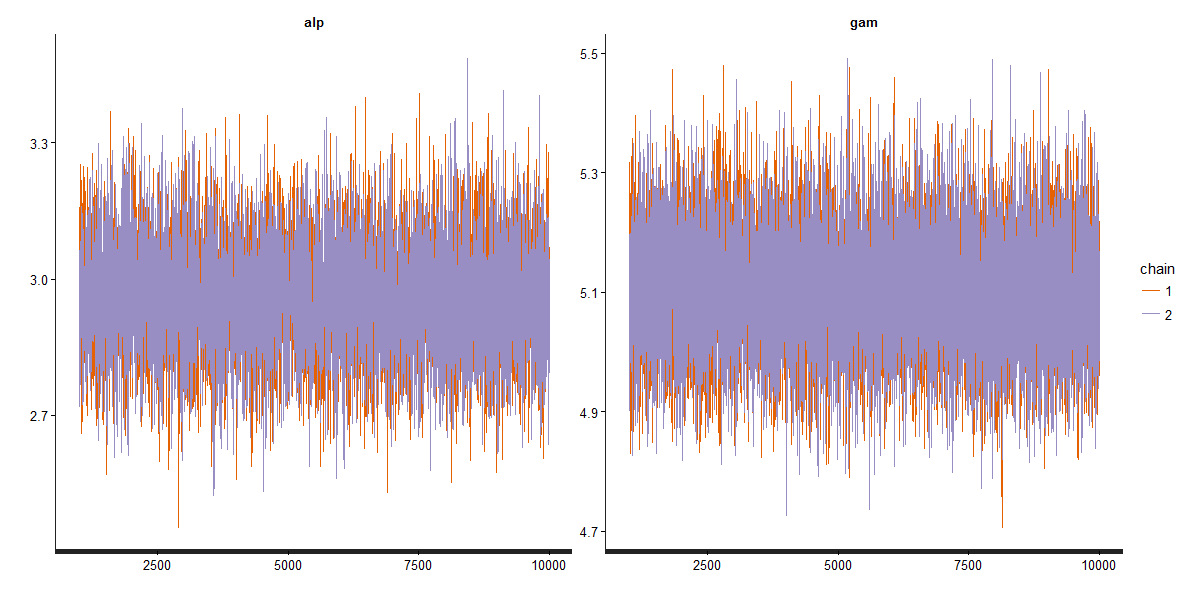
\includegraphics[width=350pt]{img/mhaz_traceplot}
    \caption{Traceplot of \lstinline{alp} and \lstinline{gam} Parameters}
    \label{mhaz_traceplot}
\end{figure}






\begin{figure}[htbp]
    \centering
    \begin{lstlisting}[belowskip=-2 \baselineskip]
generated quantities {
  vector[N] log_lik;
  for (i in 1:N){
  	log_lik[i] <- surv_dens_log(lifetime[i], alp, gam, beta_err1 * x_err1[i] + beta_err2 * x_err2[i] + beta_repair * x_repair[i] + beta_kWh * x_kWh[i] + beta_weather * park_weather[i]);
  }
}\end{lstlisting}
    \caption{Log Likelihood in Generated Quantities Block}
    \label{mhaz_loglik}
\end{figure}



Once it is clear that the model has converged to a stable solution. Fit and prediction accuracy can be assessed using WAIC and the C-Index. To generate the WAIC metric, a point-wise log likelihood, \lstinline{log_lik}, is required. Figure~\ref{mhaz_loglik} demonstrates how to retrieve this value. The \lstinline{generated quantities} block allows for these likelihoods to be extracted upon completion of sampling. The functions \lstinline{WAIC()} from the \lstinline{rethinking} package can be used to compute the WAIC value for the model under the assumption that the \lstinline{log_lik} vector is included in the output. 

To compute the C-Index, the hazard function, the prognostic measure, must first be generated. This is done by sampling the parameters from posterior. This has the added benefit of retaining the uncertainty associated with each parameter as well as the hazard function. As stated earlier, the C-Index should be computed on a hold-out sample to prevent overfitting. The simulated data used for this exploration, provides the added ability to estimate the C-Index on the uncensored lifetimes. This completes the process.

Unobserved heterogeneity or clustered observations can be implemented in several ways in Stan, with roughly the same results. However, the strategy for what is being optimized varies.

First, it is possible to repeat the mechanism with which the Multiplicative Hazard was fit, by explicitly writing out the log likelihood into the \lstinline{function} block. Recall, that the Frailty, $Z$, is not directly modeled, as it is constrained to have an expectation of one, $\mathrm{E}[Z]=1$, by design. Rather the unconditional likelihood is used with the Frailty parameter integrated out. Figure~\ref{frail_funs} illustrates the necessary changes required for the density function.


\begin{figure}[htbp]
    \centering
    \begin{lstlisting}[belowskip=-2 \baselineskip]
  real surv_dens_log(vector cens_lifetime, real alp, real gam, real sig, real lin_pred){
    real lifetime;
    real d_i;
    real sig_i;

    sig_i    <- sig;
    lifetime <- cens_lifetime[1];
    d_i      <- cens_lifetime[2];
  
    return d_i * log(sig^2) + log(tgamma((1/sig^2) + d_i)) - log(tgamma( (1/sig^2) )) -
            ((1/sig^2) + d_i) * log(1 + sig^2 * H_t(lifetime, alp, gam) * exp(lin_pred)) +
            d_i * (lin_pred + log_h_t(lifetime, alp, gam));
  }\end{lstlisting}
    \caption{Gamma Frailty Likelihood in Function Block}
    \label{frail_funs}
\end{figure}


Beyond the density function, there is also a requirement to resolve the sums across the clusters. To do this a grouping variable must be made during the model fitting process. This allows for the estimation of $\sigma^2$ for each level of the group. In this example, the each park is given its own estimate of the Frailty variance. The estimation process is done as before, but a different value is given for each of the five parks in the input data.

To do this in Stan must be made aware that the parameter \lstinline{sig} will now be a vector of real numbers. It needs to know the size of the vector. Then, the fitting process must take into account which position in the vector of \lstinline{sig} sampling is being done. Thus, the following additions are required to complete the Stan program:


\begin{figure}[htbp]
    \centering
    \begin{lstlisting}[belowskip=-2 \baselineskip]
data {
  int<lower=1>  park[N];
  int<lower=1>  park_N;
}

parameters {
  real<lower=0> sig[park_N];
}

model {
  for(i in 1:N){
      lifetime[i] ~ surv_dens(alp, gam, sig[park[i]], beta_err1 * x_err1[i] + beta_err2 * x_err2[i] + beta_repair * x_repair[i] + beta_kWh * x_kWh[i] + beta_weather * park_weather[i]);
  }
  for(j in 1:park_N){
    sig[j] ~ lognormal(0, 1.5);
  }

}\end{lstlisting}
    \caption{Park Grouping in Stan Blocks}
    \label{park_group}
\end{figure}


Figure~\ref{park_group} demonstrates the required changes. The \lstinline{data} block introduces a grouping variable, \lstinline{park} which is the length of the number of observations, \lstinline{N}. It identifies park membership of any single observation with an integer value. The \lstinline{park_N} variable is introduced to provide a count of the total number of parks in the whole dataset. This is useful in the \lstinline{parameters} block for defining the dimensions of the \lstinline{sig} vector that stores the variances of the Frailty parameter. Finally, in the \lstinline{model} block, the same sampling statement is made as before, however, now the additional indexing of the \lstinline{sig} parameter is introduced. This is done through the use of an index on the \lstinline{park} variable, which has a range between one and five. As such, when the sampling statement is run, a value at each park is generated within, \lstinline{sig[park[i]]}.


\begin{figure}[htbp]
    \centering
    \begin{lstlisting}[belowskip=-2 \baselineskip]
  real surv_dens_log(vector cens_lifetime, real alp, real gam, real lin_pred, real Z){
    real lifetime;
    real d_i;
  
    lifetime <- cens_lifetime[1];
    d_i      <- cens_lifetime[2];
  
    return d_i * (log_h_t(lifetime, alp, gam) + lin_pred + Z) - (H_t(lifetime, alp, gam) * exp(lin_pred) * exp(Z));
  }\end{lstlisting}
    \caption{Fraily Model with Direct Estimation of $Z$ parameter}
    \label{z_lik}
\end{figure}


An alternative method can be used to fit the model in a substantially more flexible and extensible form. This allows for the direct sampling of the $Z$ parameter rather than integrating it out through a constraint. This greatly simplifies the model. Figure~\ref{z_lik} provides the likelihood function, \lstinline{surv_dens_log}, needed to fit the model. The other alterations required to the code are the same as in in the previous case, a vector of $Z$ parameters must be defined in the \lstinline{parameter} block and added to the end of the likelihood function call in the \lstinline{model} block. As before, a park grouping should be used like \lstinline{Z[park[i]] to ensure the sampling is done for each park. As can be seen from Figure~\ref{z_lik}, the introduction of the $Z$ parameter simply requires the inclusion of a single term to the hazard and cumulative hazard of the likelihood. This likelihood is the original simple likelihood of the Multiplicative Hazard Model. 

\begin{figure}[htbp]
    \centering
    \begin{lstlisting}[belowskip=-2 \baselineskip]
              mean se_mean   sd  2.5%   25%   50%   75% 97.5% n_eff Rhat
alp           2.92    0.00 0.19  2.55  2.79  2.92  3.06  3.30  6818    1
gam           6.79    0.01 0.83  5.57  6.22  6.65  7.22  8.77  5811    1
Z[1]          0.57    0.01 0.47  0.02  0.21  0.46  0.80  1.78  6111    1
Z[2]          0.48    0.01 0.38  0.02  0.19  0.39  0.67  1.46  5266    1
Z[3]          0.97    0.01 0.37  0.31  0.72  0.95  1.20  1.79  5253    1
Z[4]          0.41    0.00 0.33  0.01  0.16  0.34  0.58  1.23  6143    1
Z[5]          0.48    0.00 0.38  0.02  0.19  0.39  0.67  1.45  5938    1
beta_err1     0.01    0.00 0.10 -0.18 -0.05  0.01  0.08  0.20 12254    1
beta_err2     2.78    0.00 0.18  2.44  2.66  2.78  2.90  3.13  6978    1
beta_repair  -0.16    0.00 0.10 -0.36 -0.23 -0.16 -0.10  0.03 13082    1
beta_kWh     -3.87    0.00 0.25 -4.36 -4.03 -3.87 -3.70 -3.39  6733    1
beta_weather  0.19    0.00 0.27 -0.35  0.02  0.18  0.35  0.77  6185    1\end{lstlisting}
    \caption{Output of Frailty Model}
    \label{out_frail}
\end{figure}

Figure~\ref{out_frail} provides the standard output for the Frailty model. As before, it includes what is expected, the mean values of the posterior, standard errors, the distributions standard deviations and quantiles for each parameter. Additionally, the $Z$ parameters are presented which express the hazard at each park. The larger than average value of \lstinline{Z[3]} illustrates that there is some systemic problem at that park that maintenance staff may wish to address. While the structure of the model, not the output, improves the prediction, the ability to understand the rationale for those predictions is a valuable tool for enabling better decision making about how to allocate resources.

This completes the shared Frailty extension. The remainder of the process is identical to that which was performed above. Upon completion the basic sanity check of statistical modeling must be performed. Assumptions regarding the adequacy of the baseline hazard and the convergence of the model should be checked in the same manner as described before. The C-Index and WAIC should be used to check the predictive performance as well as to ensure that the model is not overfitting. Finally, a list of the most at-risk inverters can be output.

One of the wondrous benefits of working with Stan, is that the models constructed above can be extended indefinitely with simple additions. This can be done in the same manner as presented previously through the addition of Frailties to deal with unobserved heterogeneity. Numerous potential extensions are feasible, only an understanding of their structural affect must be integrated. For example, it is possible to stratify the baseline hazard allowing a different shape and scale for each group. It is also possible to expand the Frailty beyond the current independence assumption and provide a correlation structure between terms in the model. It is even possible to directly model time-varying effects, to explicitly cope with phenomena whose relationship changes as the system ages. The possibilities need only to be justified, tested and checked to ensure they provide improvements in out of sample performance. The extension potential is limitless. 






\section*{Extended Reading}
\addcontentsline{toc}{section}{Extended Reading}


For an excellent guide to feature engineering of time-dependent processes, the reader is directed to Microsoft Playbook by Uz\cite{Uz2016}. Inverse transform sampling in time-to-event models is covered by Bender, Augustin and Blettner\cite{Bender2005}, is extended to Frailties by Romdhane and Belkacem\cite{Romdhane2015} and into time-dependent covariates by Austin\cite{Austin2012} and Hendry\cite{Hendry2014}. For more information on the Stan probabilistic programming language, the Stan development team has a exhaustive manual in place\cite{StanDevelopmentTeam2016}. For development of measures to assess the accuracy of predictive models or any models, the classic text by Harrell is highly recommended\cite{Harrell2001}. For more information about WAIC, Vehtari, Gelman and Garby cover the derivation and properties\cite{Vehtari2015}. For an overview of how to implement models in Stan, the massive Stan Reference Manual is likely without equal\cite{StanDevelopmentTeam2016}. For slightly less overwhelming information about Stan, the documentation page on the project website contains a wide assortment of tutorials, videos and softer introductions to the software\cite{StanDevelopmentTeam2016a}.


